\documentclass[10pt]{beamer}
\usetheme{Boadilla}

\definecolor{cyberdark}{RGB}{15, 23, 42}
\definecolor{cybergray}{RGB}{51, 65, 85}
\definecolor{cyberblue}{RGB}{37, 99, 235}
\definecolor{cyberpurple}{RGB}{124, 58, 237}

\setbeamercolor{palette primary}{bg=cyberdark, fg=white}
\setbeamercolor{palette secondary}{bg=cybergray, fg=white}
\setbeamercolor{palette tertiary}{bg=cyberblue, fg=white}
\setbeamercolor{palette quaternary}{bg=cyberpurple, fg=white}
\setbeamercolor{structure}{fg=cyberblue}
\setbeamercolor{item}{fg=cyberpurple}

\title[Network Anomaly Detection]{Anomaly Detection in Network Traffic}
\subtitle{A Machine Learning Approach -- Deliverable 3}
\author[Group 1]{Gon\c{c}alo Almeida \and Margarida Ribeiro \and Jo\~{a}o Barreira}
\institute[Univ. Aveiro]{Universidade de Aveiro}
\date[May 2026]{May 29, 2026}

\begin{document}

\begin{frame}
  \titlepage
\end{frame}

% ─────────────────────────────────────────────────────────────
% PART 1: Jo\~{a}o Barreira (Pipeline & EDA)
% ─────────────────────────────────────────────────────────────

\begin{frame}{Context and Dataset (CIC-IDS2017)}
  \begin{itemize}
    \item \textbf{Cybersecurity Challenge:} Identifying malicious traffic dynamically.
    \item \textbf{Dataset Selection:} Canadian Institute for Cybersecurity (CIC-IDS2017).
    \begin{itemize}
      \item Realistic normal traffic mixed with modern multi-vector attacks (DDoS, Brute Force, Web Attacks, etc.).
    \end{itemize}
    \item \textbf{Computational Hurdles:}
    \begin{itemize}
      \item Over \textbf{2.8 million instances} ($>1$ GB raw CSVs) triggering OOM errors on local machines.
      \item Severe class imbalance: \textbf{80.3\% benign} vs. \textbf{19.7\% anomalous}.
    \end{itemize}
  \end{itemize}
\end{frame}

\begin{frame}{Exploratory Data Analysis (EDA)}
  \begin{columns}
    \begin{column}{0.5\textwidth}
      \textbf{Key Insights:}
      \begin{itemize}
        \item Highly skewed attributes (Flow Duration: $\mu$s to $\ge 100$s).
        \item Strong correlations detected between packet volumes and rate features.
        \item Identified 8 static features (zero-variance) that were pruned.
      \end{itemize}
    \end{column}
    \begin{column}{0.5\textwidth}
      \centering
      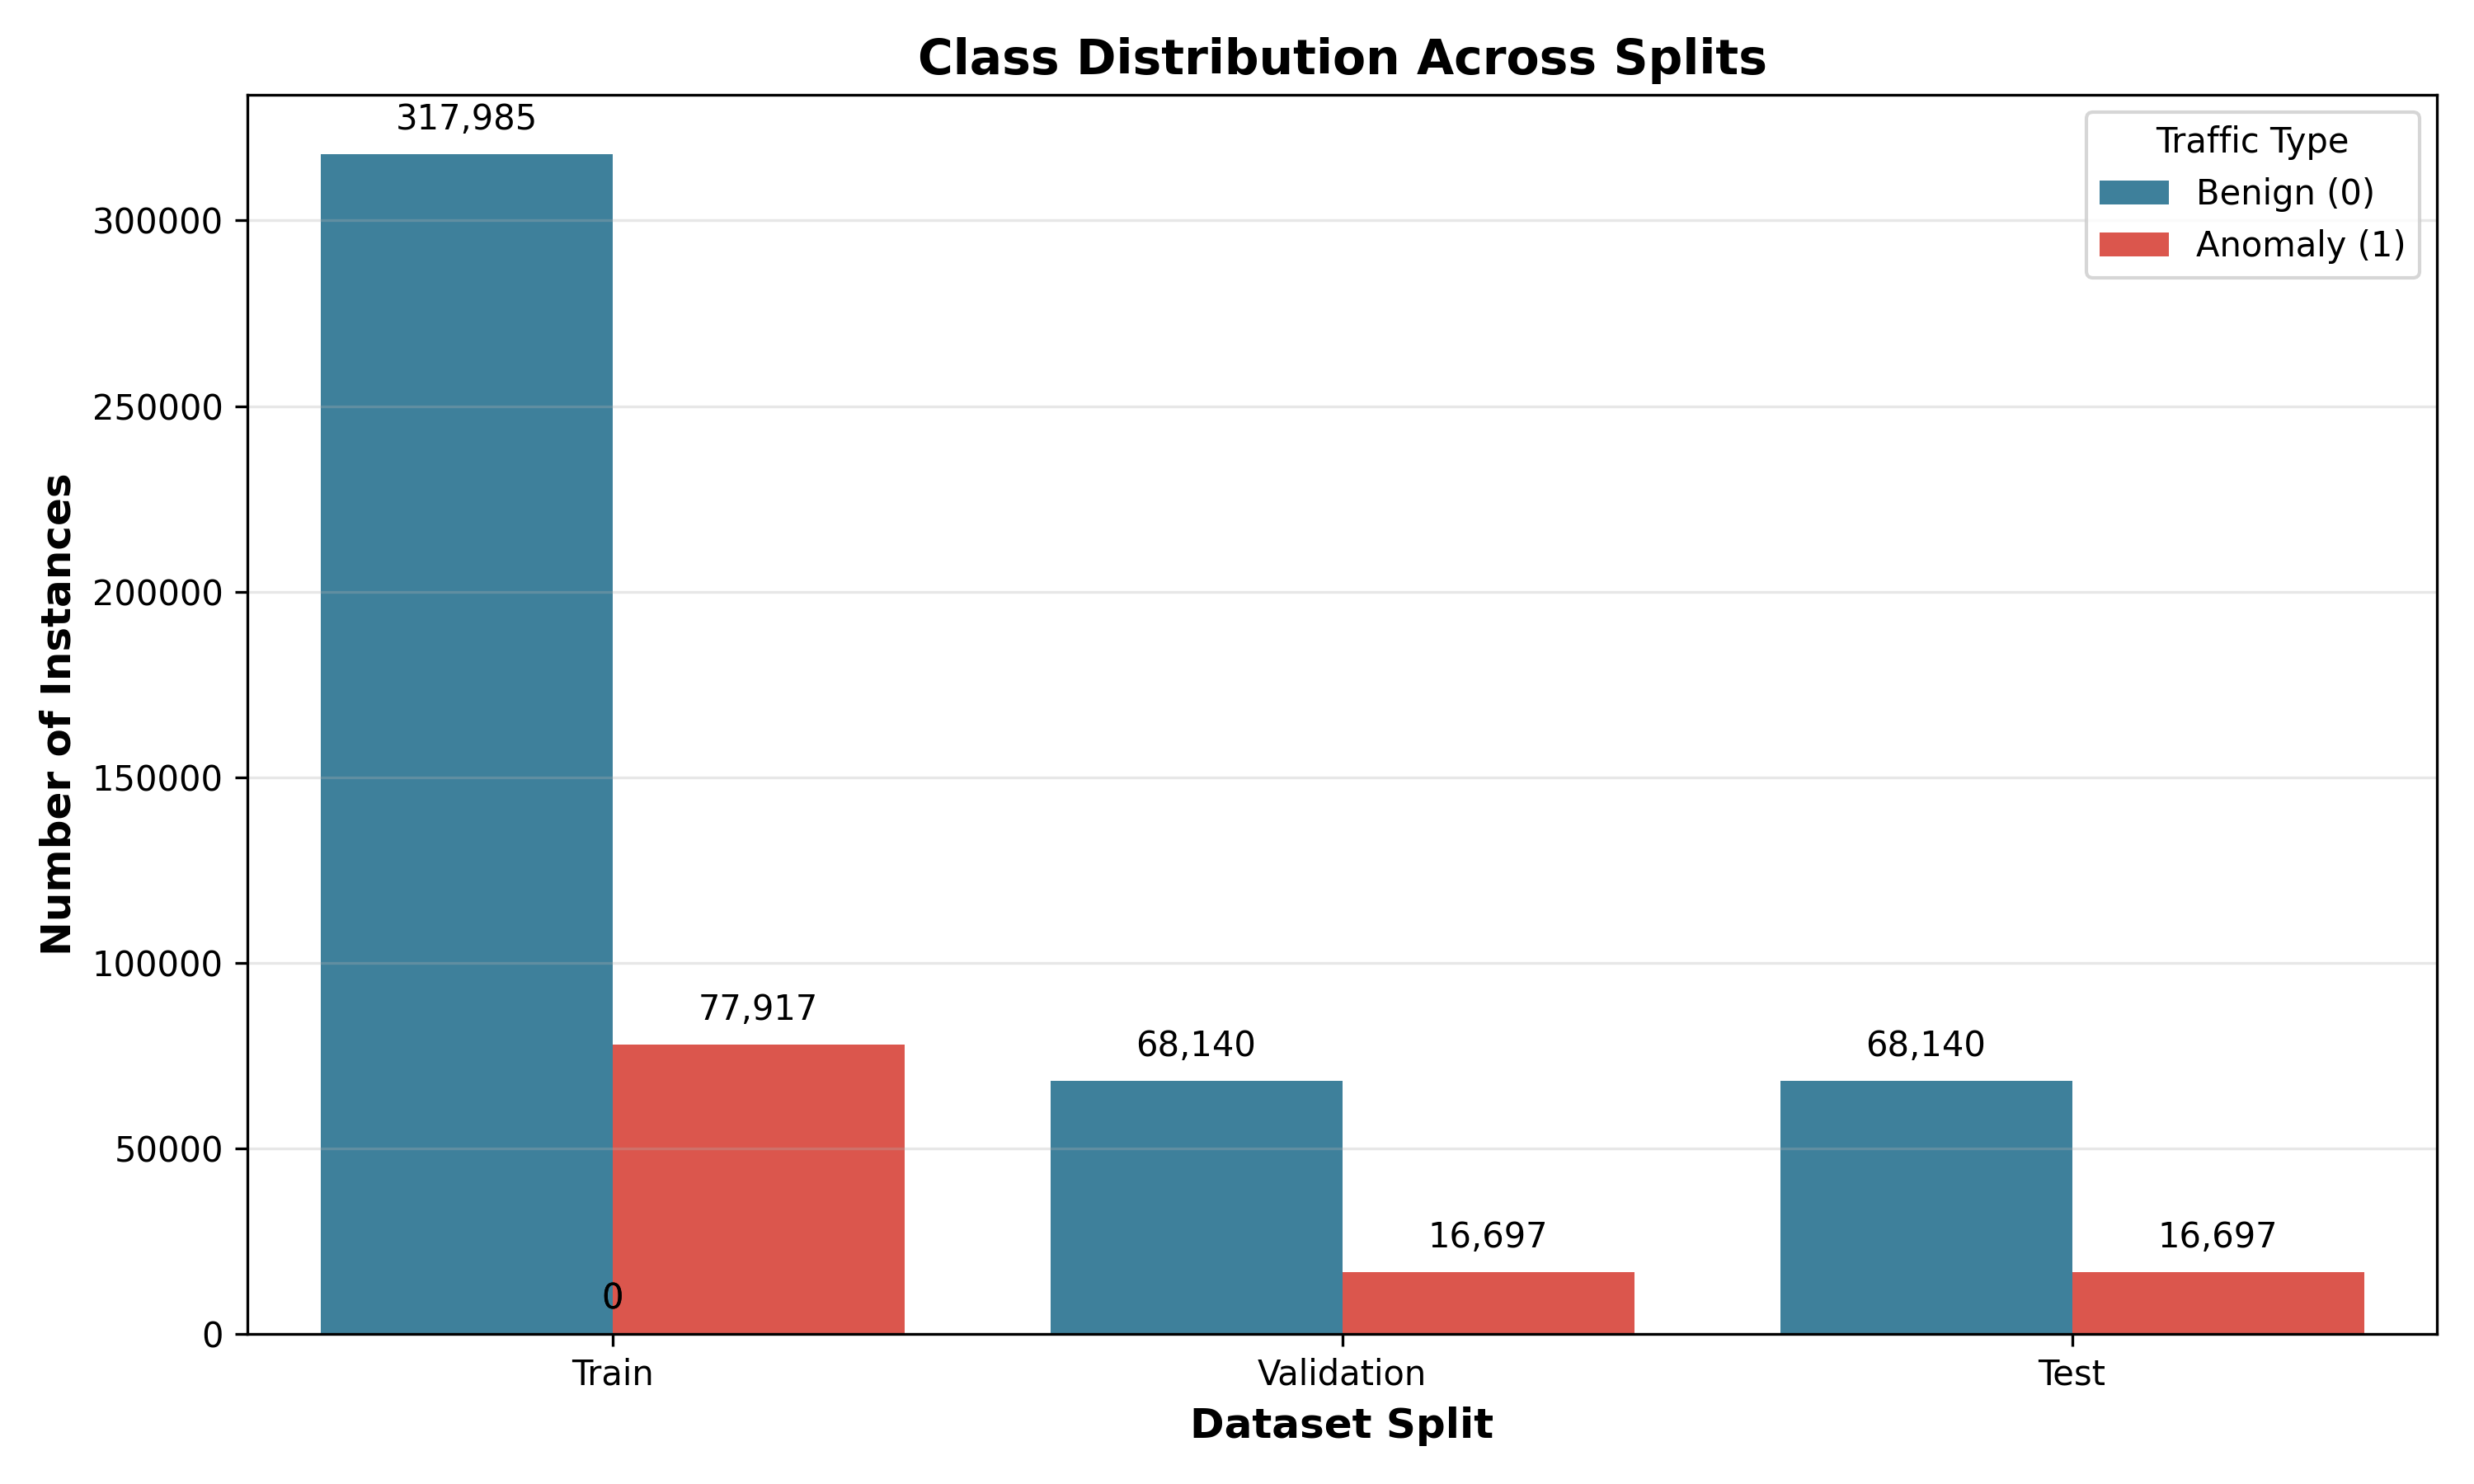
\includegraphics[width=0.9\textwidth]{images/class_distribution.png}\\
      \scriptsize{Native 80/20 Class Distribution}
    \end{column}
  \end{columns}
\end{frame}

\begin{frame}{Data Preprocessing Pipeline}
  \begin{enumerate}
    \item \textbf{Data Cleaning:} Handled column header whitespaces, dropped NaN and Infinite values ($<0.1\%$ impact).
    \item \textbf{Feature Selection:} Dropped zero-variance variables (e.g., \texttt{Bwd PSH Flags}) to reduce computational noise.
    \item \textbf{Stratified Sampling:} Extracted a representative 20\% sample ($\approx 565,000$ rows) maintaining the 80/20 class split.
    \item \textbf{Split \& Scale:} 70/15/15 train/val/test split. Normalization using \textit{StandardScaler} fitted strictly on training data to prevent \textbf{data leakage}.
  \end{enumerate}
\end{frame}

\begin{frame}{Evaluation Strategy}
  \begin{itemize}
    \item \textbf{Imbalance Impact:} Traditional accuracy is misleading (always predicting 'normal' achieves 80.3\% accuracy).
    \item \textbf{Selected Metrics:} F1-Score, Recall (critical to catch all attacks), Precision, and AUC-ROC.
    \item \textbf{Multi-Perspective Framework:}
    \begin{enumerate}
      \item \textbf{Original Distribution:} Realistic test environment.
      \item \textbf{Balanced Subset (50-50):} Exposes pure algorithm discrimination.
      \item \textbf{Per-Class Breakdown:} Recall analysis across different attack vectors.
    \end{enumerate}
  \end{itemize}
\end{frame}

% ─────────────────────────────────────────────────────────────
% PART 2: Margarida Ribeiro (SOTA & Classical Models)
% ─────────────────────────────────────────────────────────────

\begin{frame}{State of the Art in Network Anomaly Detection}
  \begin{table}
    \centering
    \caption{Summary of literature models and findings.}
    \label{tab:sota_slides}
    \scriptsize
    \begin{tabular}{lllr}
      \hline
      \textbf{Method} & \textbf{Type} & \textbf{Data Benchmark} & \textbf{AUC} \\ \hline
      Isolation Forest (2008) & Tree Ensemble & KDD'99 & 0.96 \\
      LOF (2000) & Density Ratio & Synthetic & 0.89 \\
      One-Class SVM (2001) & Kernel Boundary & USPS & 0.87 \\
      Autoencoder (2014) & Deep learning & MSDS & 0.93 \\
      Kitsune (2018) & Ensemble AE & Real Traffic & 0.99 \\
      DAGMM (2018) & Deep Hybrid & KDD'99 & 0.98 \\ \hline
    \end{tabular}
  \end{table}
  \textbf{Major Conclusions from Review:}
  \begin{itemize}
    \item Tree ensembles and neural networks consistently outperform density methods in dimensions $>20$.
    \item Hyperparameter tuning is rarely reported systematically in cybersecurity papers.
  \end{itemize}
\end{frame}

\begin{frame}{Classical Algorithms Evaluated}
  \begin{itemize}
    \item \textbf{Isolation Forest:} Builds an ensemble of isolation trees. Anomalies are isolated closer to the root of the trees.
    \item \textbf{One-Class SVM:} Constructs a maximum-margin hyperplane in a high-dimensional kernel space to separate normal points.
    \item \textbf{Local Outlier Factor (LOF):} Compares the local reachability density of a point against its $k$-nearest neighbors.
  \end{itemize}
  \vfill
  \textbf{Hyperparameter tuning strategy:}
  \begin{itemize}
    \item \textbf{3-Fold Stratified Cross-Validation (CV)} conducted on the training split to select optimal parameters.
    \item Fixed held-out test set preserved strictly for final comparisons.
  \end{itemize}
\end{frame}

\begin{frame}{Classical Models Tuning Heatmaps}
  \begin{columns}
    \begin{column}{0.5\textwidth}
      \centering
      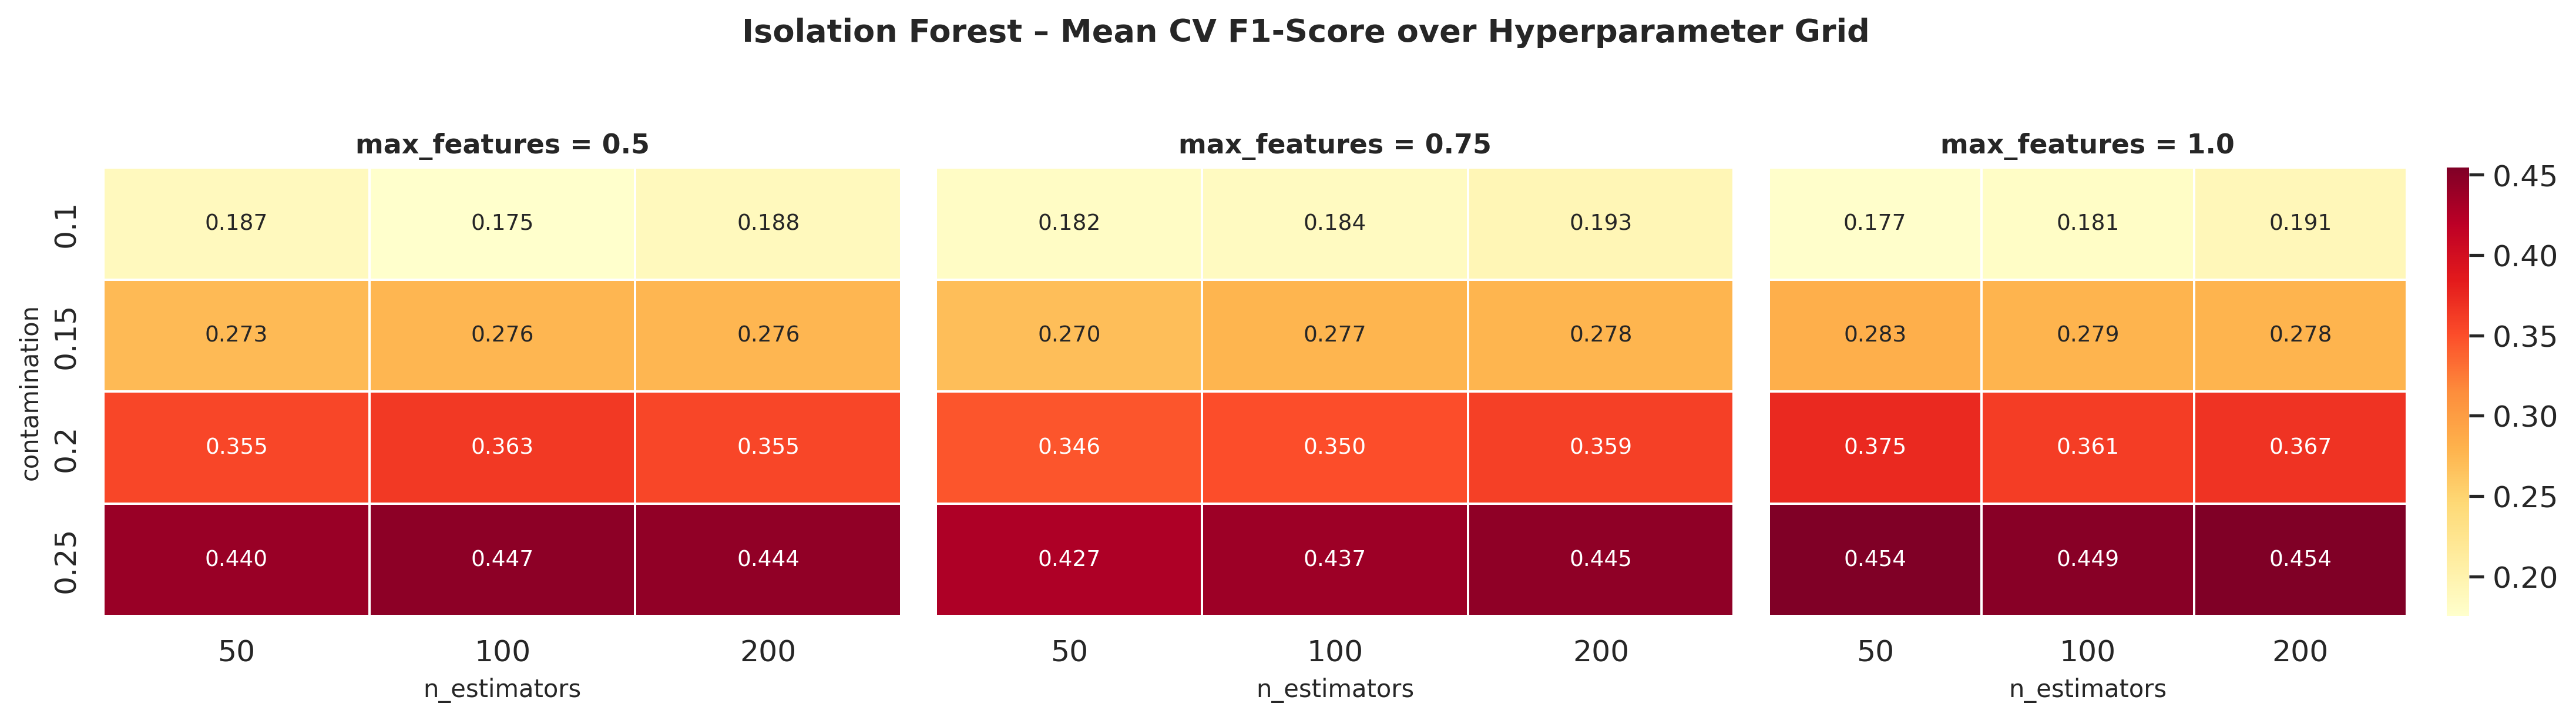
\includegraphics[width=0.85\textwidth]{../tuning_results/if_heatmap.png}\\
      \scriptsize{Isolation Forest CV F1-Score}
    \end{column}
    \begin{column}{0.5\textwidth}
      \centering
      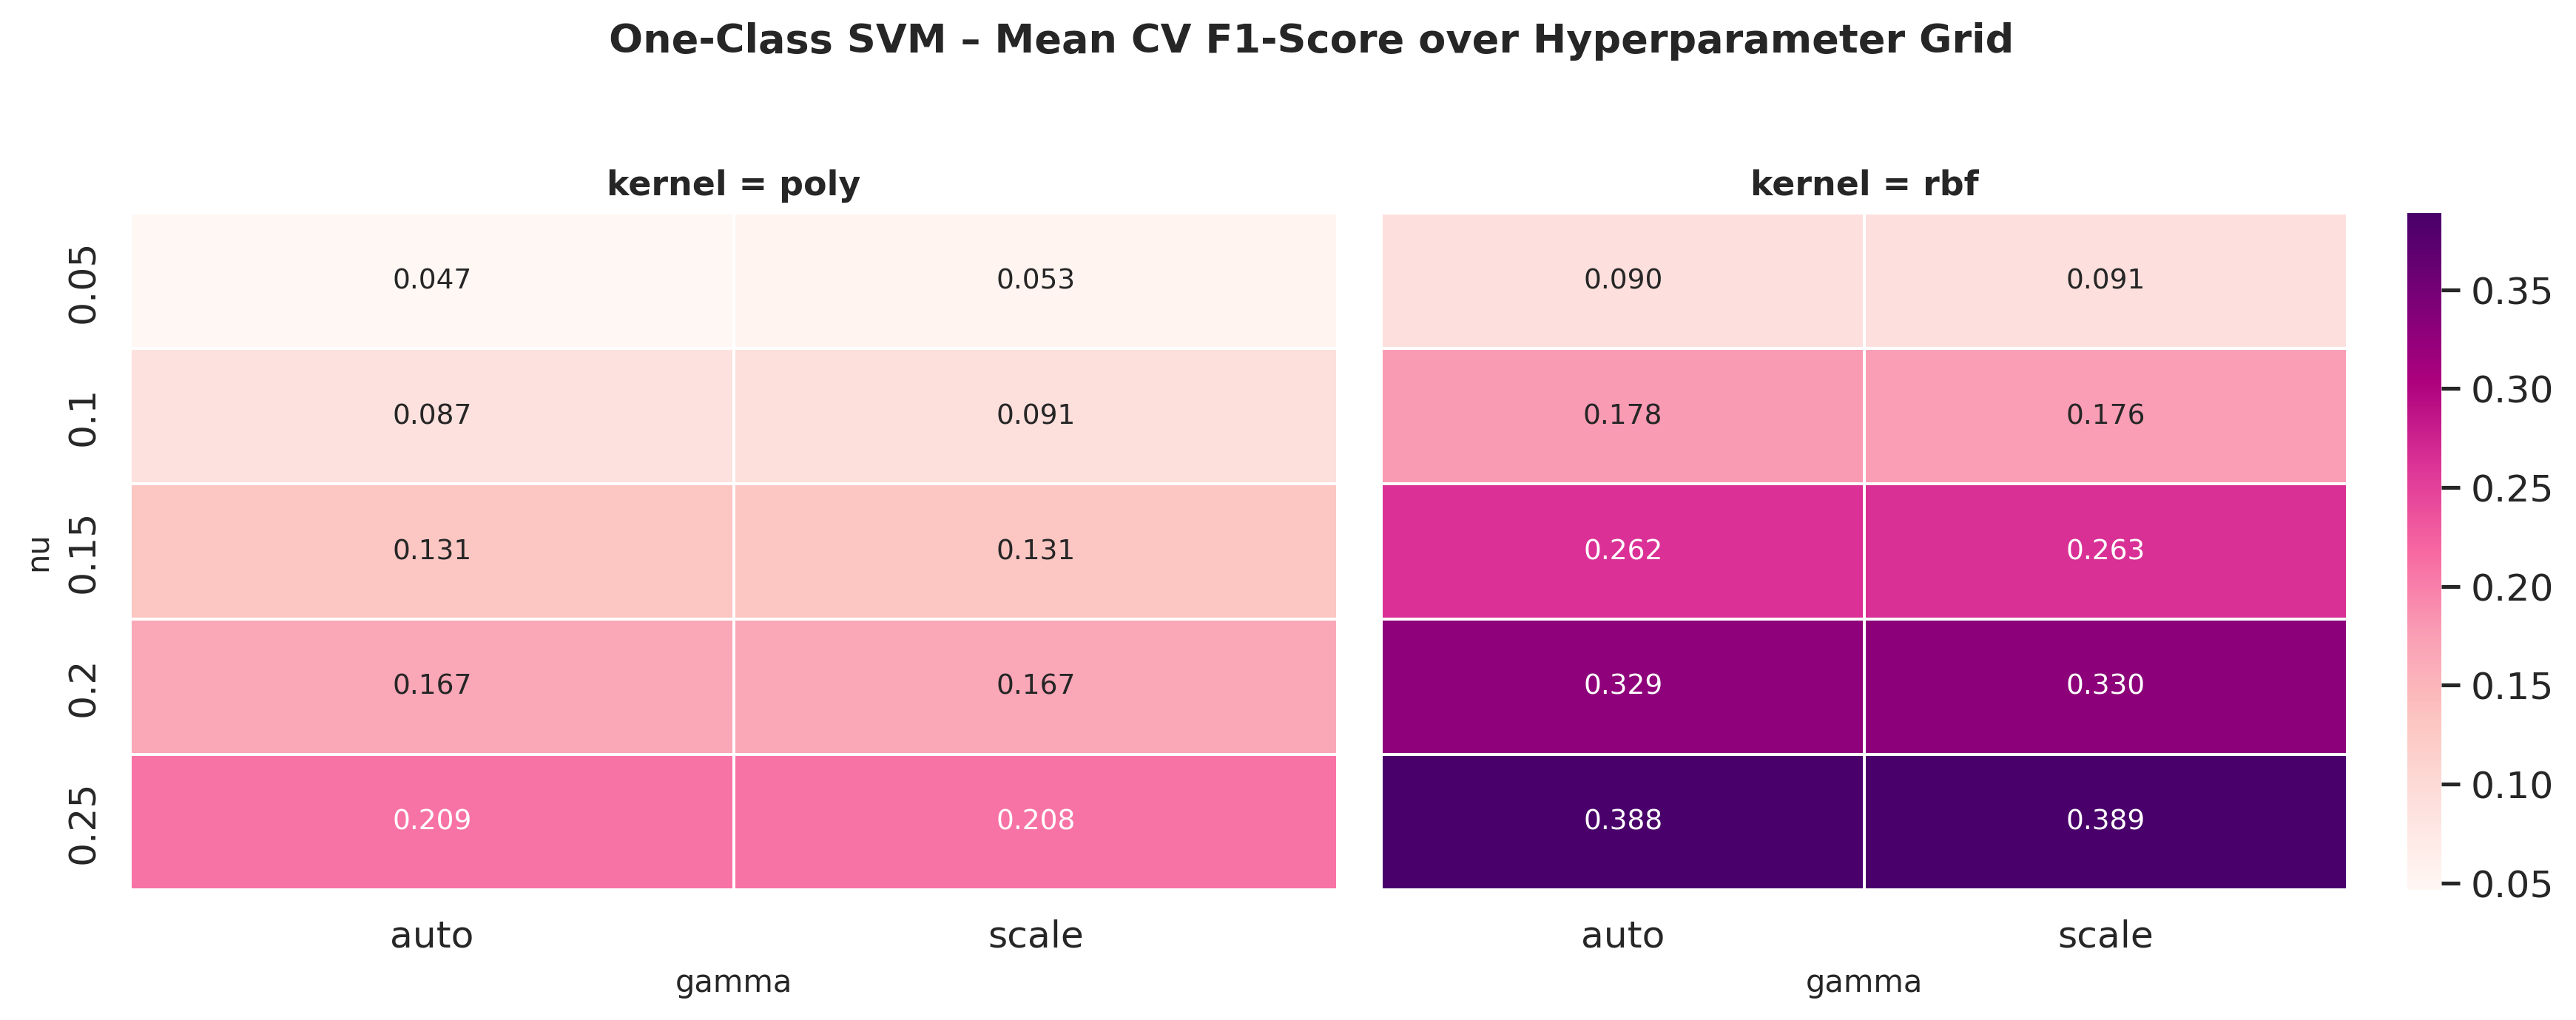
\includegraphics[width=0.85\textwidth]{../tuning_results/ocsvm_heatmap.png}\\
      \scriptsize{One-Class SVM (RBF vs. Poly) CV F1}
    \end{column}
  \end{columns}
  \vfill
  \begin{itemize}
    \item \textbf{Isolation Forest:} Contamination is the most sensitive parameter.
    \item \textbf{One-Class SVM:} RBF kernel consistently beats Polynomial.
  \end{itemize}
\end{frame}

\begin{frame}{Baseline vs. Tuned Performance}
  \begin{columns}
    \begin{column}{0.5\textwidth}
      \centering
      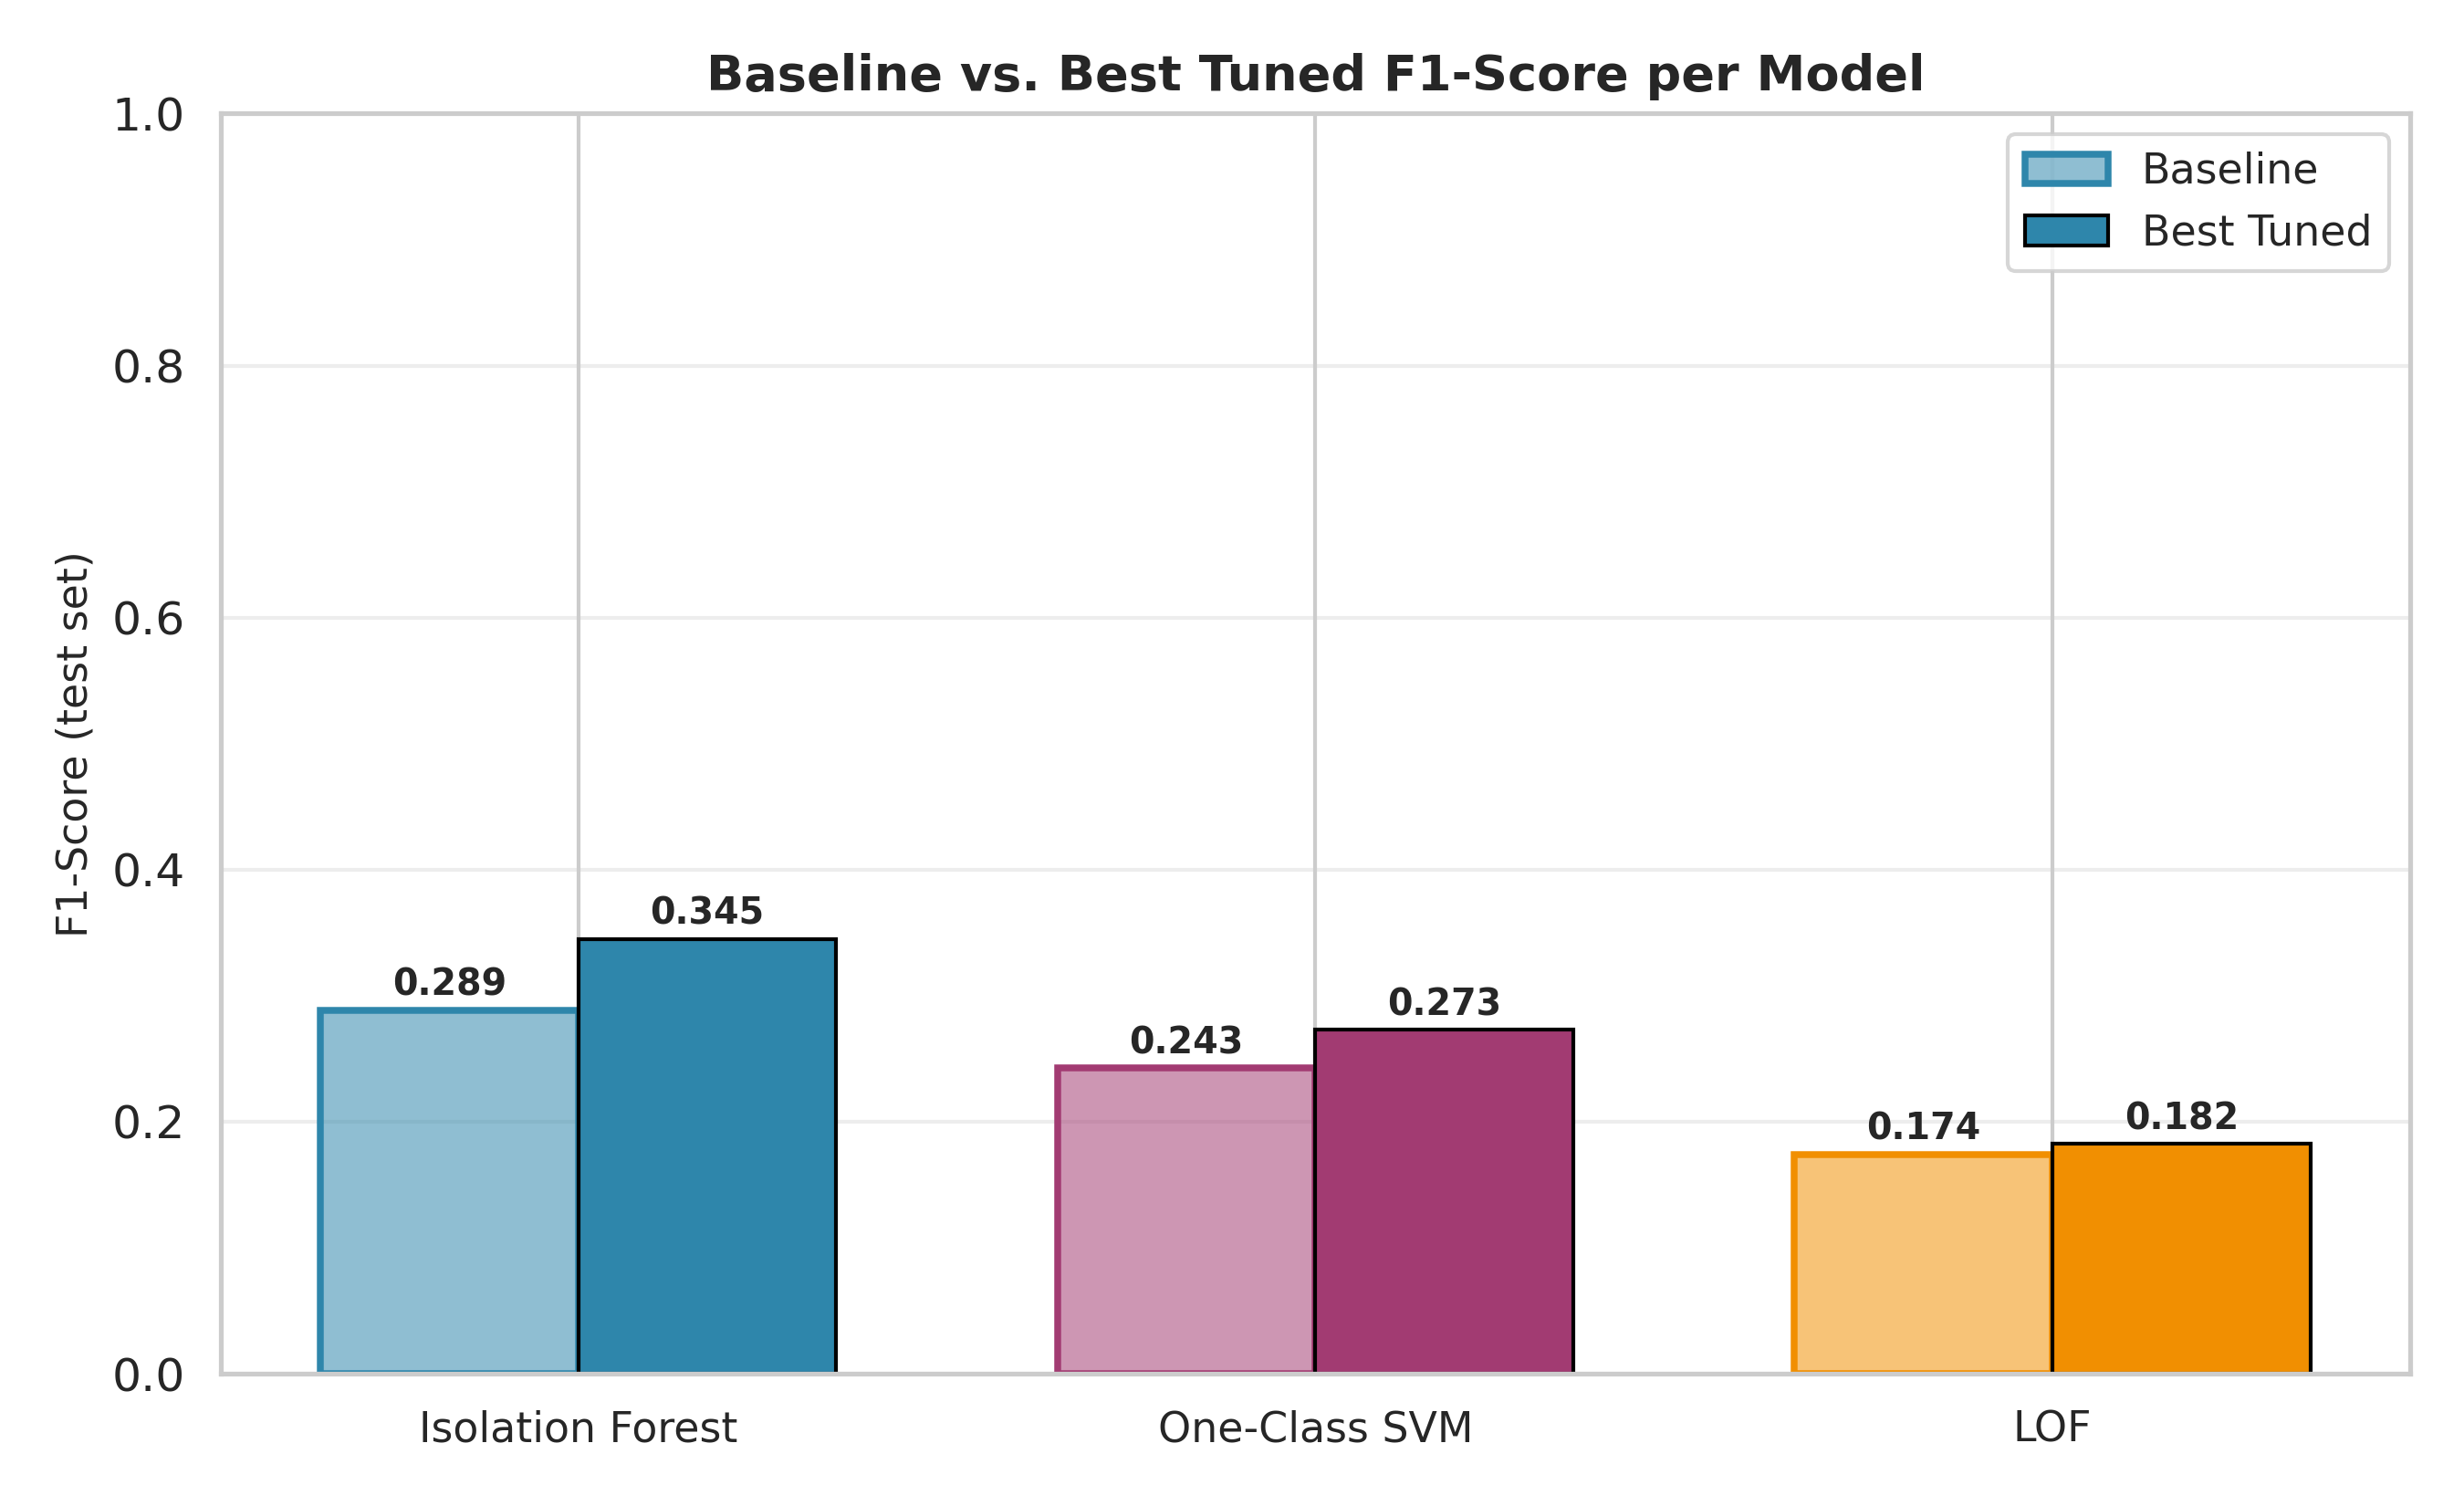
\includegraphics[width=0.9\textwidth]{../tuning_results/baseline_vs_best.png}\\
      \scriptsize{Test F1 Comparison (Baseline vs. Best)}
    \end{column}
    \begin{column}{0.5\textwidth}
      \textbf{Results of Tuning:}
      \begin{itemize}
        \item \textbf{Isolation Forest:} Significant boost from tuning ($+5.6\%$ F1 score).
        \item \textbf{One-Class SVM:} Moderate improvement ($+3.0\%$ F1).
        \item \textbf{LOF:} Negligible change. Confirming that LOF's density ratios break down in high-dimensional (70D) spaces.
      \end{itemize}
    \end{column}
  \end{columns}
\end{frame}

% ─────────────────────────────────────────────────────────────
% PART 3: Gon\c{c}alo Almeida (Deep Learning, Results & Reflection)
% ─────────────────────────────────────────────────────────────

\begin{frame}{Deep Learning Architectures (Autoencoders)}
  \begin{itemize}
    \item \textbf{Primary Autoencoder (Normal-Trained):}
    \begin{itemize}
      \item Trained exclusively on benign network traffic ($y=0$).
      \item Reconstruction MSE loss: $\mathcal{L}_{\text{MSE}} = \frac{1}{N} \sum \|\mathbf{x} - \mathbf{\hat{x}}\|^2$.
      \item Anomaly Score: $s_{\text{primary}}(\mathbf{x}) = \|\mathbf{x} - \mathbf{\hat{x}}\|^2$.
    \end{itemize}
    \item \textbf{Secondary Autoencoder (Anomaly-Trained):}
    \begin{itemize}
      \item Trained exclusively on malicious traffic ($y=1$).
      \item Learns statistical similarities of attacks.
      \item Anomaly Score: $s_{\text{secondary}}(\mathbf{x}) = -\|\mathbf{x} - \mathbf{\hat{x}}_2\|^2$.
    \end{itemize}
    \item \textbf{Ensemble Autoencoder:}
    \begin{itemize}
      \item Logical OR-gate decision framework: $\hat{y}_{\text{ensemble}} = \hat{y}_{\text{primary}} \lor \hat{y}_{\text{secondary}}$.
      \item Maximizes detection rates, minimizing dangerous false negatives.
    \end{itemize}
  \end{itemize}
\end{frame}

\begin{frame}{Autoencoders Training Convergence}
  \begin{columns}
    \begin{column}{0.6\textwidth}
      \centering
      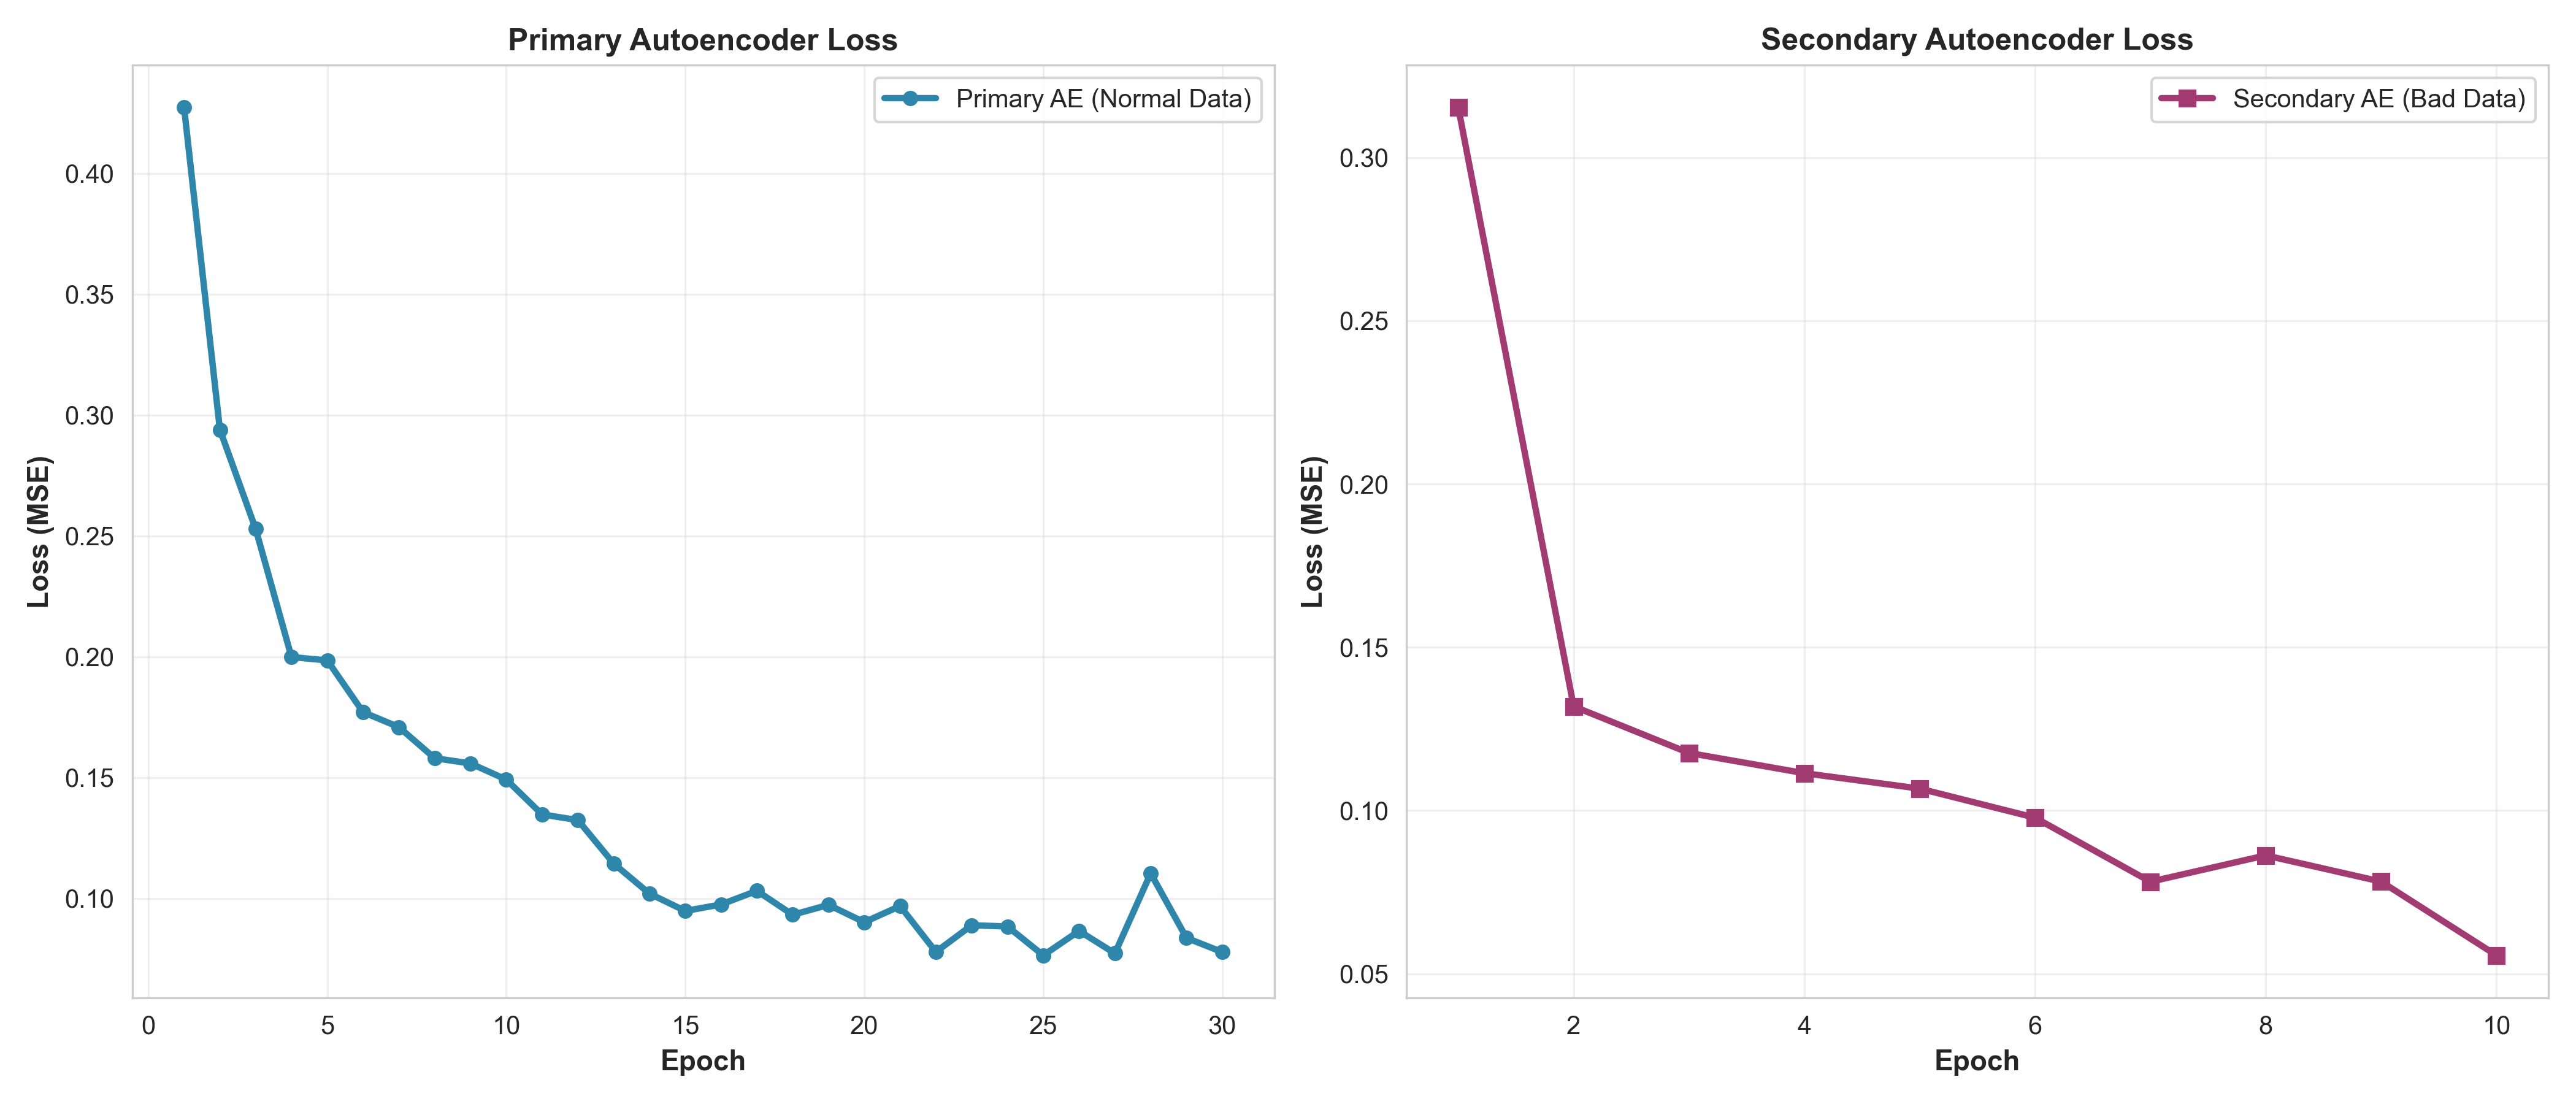
\includegraphics[width=0.9\textwidth]{images/autoencoder_loss_comparison.png}\\
      \scriptsize{Training Loss curves for both network branches}
    \end{column}
    \begin{column}{0.4\textwidth}
      \textbf{Convergence Analysis:}
      \begin{itemize}
        \item Primary AE converged smoothly within 30 epochs (final MSE: 0.0615).
        \item Secondary AE converged quickly (10 epochs) due to structured attack patterns.
        \item No overfitting observed on validation set.
      \end{itemize}
    \end{column}
  \end{columns}
\end{frame}

\begin{frame}{Final Metric Comparison (Test Set)}
  \begin{table}
    \centering
    \caption{Model results under original and balanced test splits.}
    \scriptsize
    \begin{tabular}{l|ccc|ccc}
      \hline
      & \multicolumn{3}{c|}{\textbf{Original (Imbalanced)}} & \multicolumn{3}{c}{\textbf{Balanced (50-50)}} \\
      \textbf{Model} & \textbf{Precision} & \textbf{Recall} & \textbf{F1} & \textbf{Precision} & \textbf{Recall} & \textbf{F1} \\ \hline
      Isolation Forest & 0.4522 & 0.4625 & 0.4573 & 0.7770 & 0.4625 & 0.5798 \\
      One-Class SVM & 0.3844 & 0.3943 & 0.3893 & 0.7159 & 0.3943 & 0.5085 \\
      LOF & 0.1327 & 0.1372 & 0.1349 & 0.3902 & 0.1372 & 0.2030 \\
      Autoencoder & 0.5545 & 0.5635 & 0.5589 & 0.8366 & 0.5635 & 0.6734 \\
      Second AE & \textbf{0.7781} & 0.7907 & \textbf{0.7844} & \textbf{0.9375} & 0.7907 & 0.8579 \\
      \textbf{Ensemble AE} & 0.5855 & \textbf{0.9530} & 0.7253 & 0.8505 & \textbf{0.9530} & \textbf{0.8989} \\ \hline
    \end{tabular}
  \end{table}
  \begin{itemize}
    \item \textbf{Deep Learning Dominance:} PyTorch Autoencoders far exceed classical.
    \item \textbf{Ensemble AE:} Best recall (\textbf{95.3\%}) and AUC-ROC (\textbf{0.981}), crucial for maximum security.
    \item \textbf{Second AE:} Best precision (\textbf{77.81\%} original) and F1 (\textbf{0.7844}), minimizing false alarms.
  \end{itemize}
\end{frame}

\begin{frame}{Ensemble Diagnostics}
  \begin{columns}
    \begin{column}{0.5\textwidth}
      \centering
      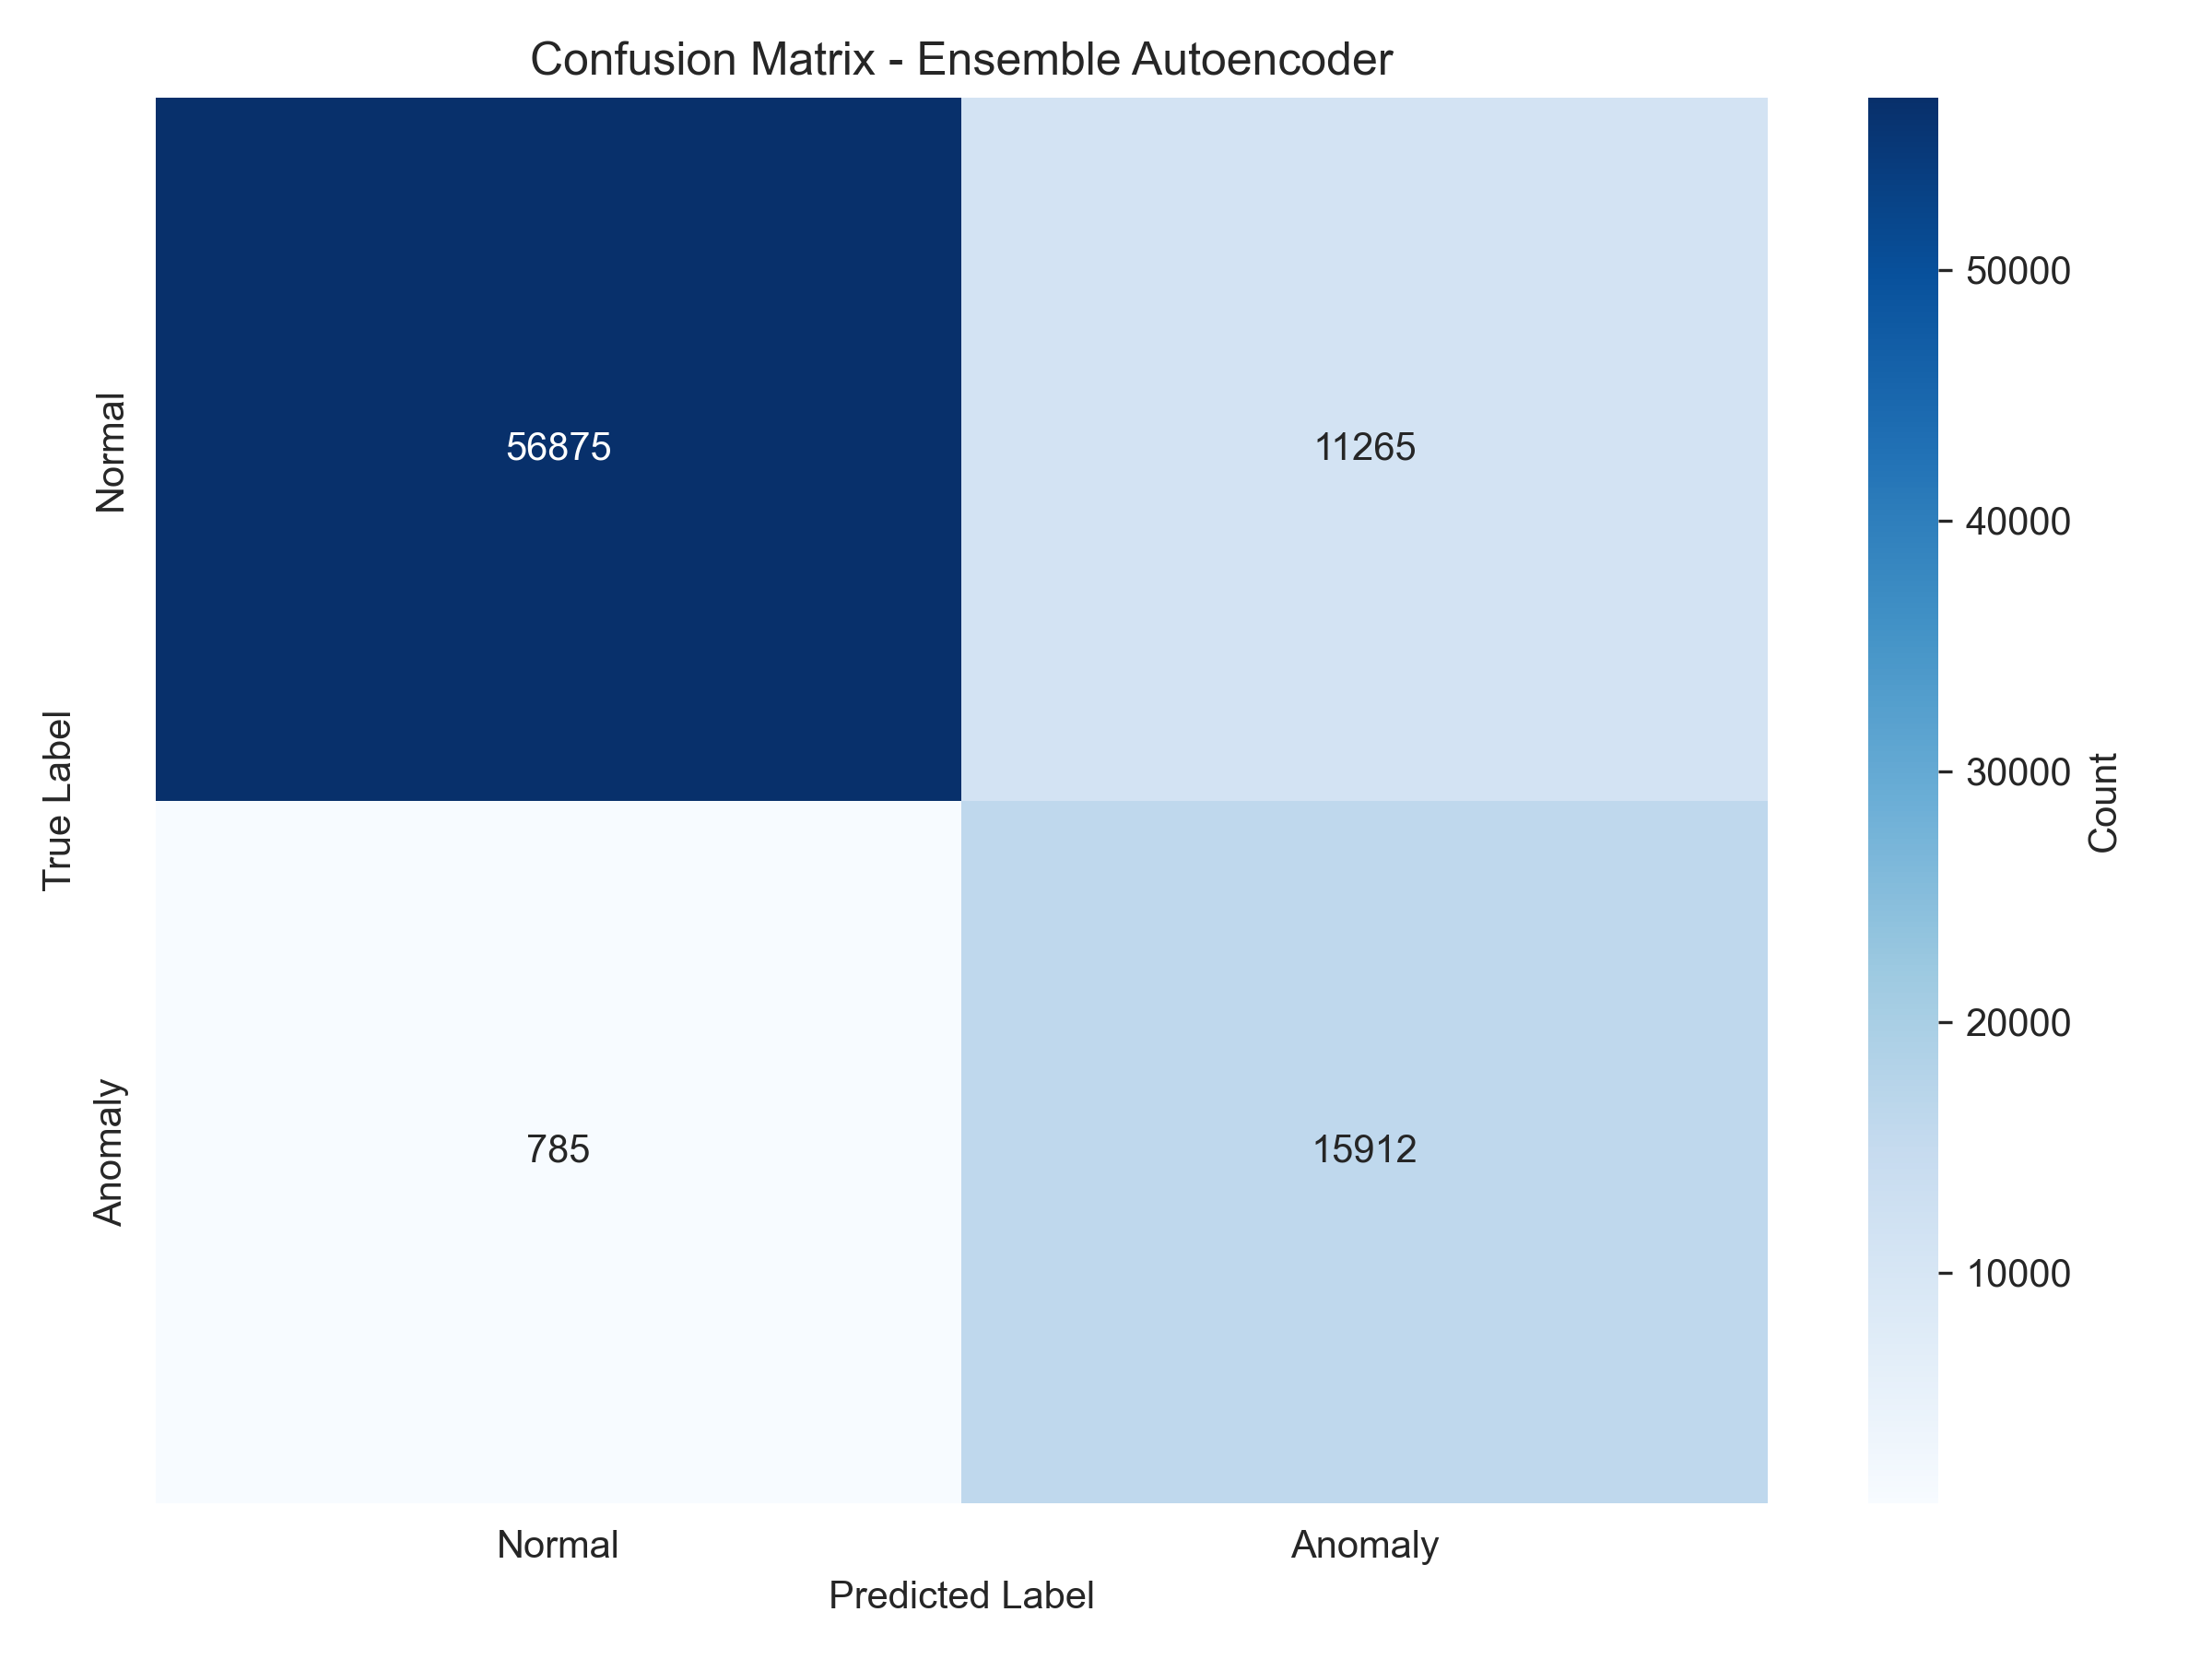
\includegraphics[width=0.85\textwidth]{images/ensemble_autoencoder_cm.png}\\
      \scriptsize{Confusion Matrix}
    \end{column}
    \begin{column}{0.5\textwidth}
      \centering
      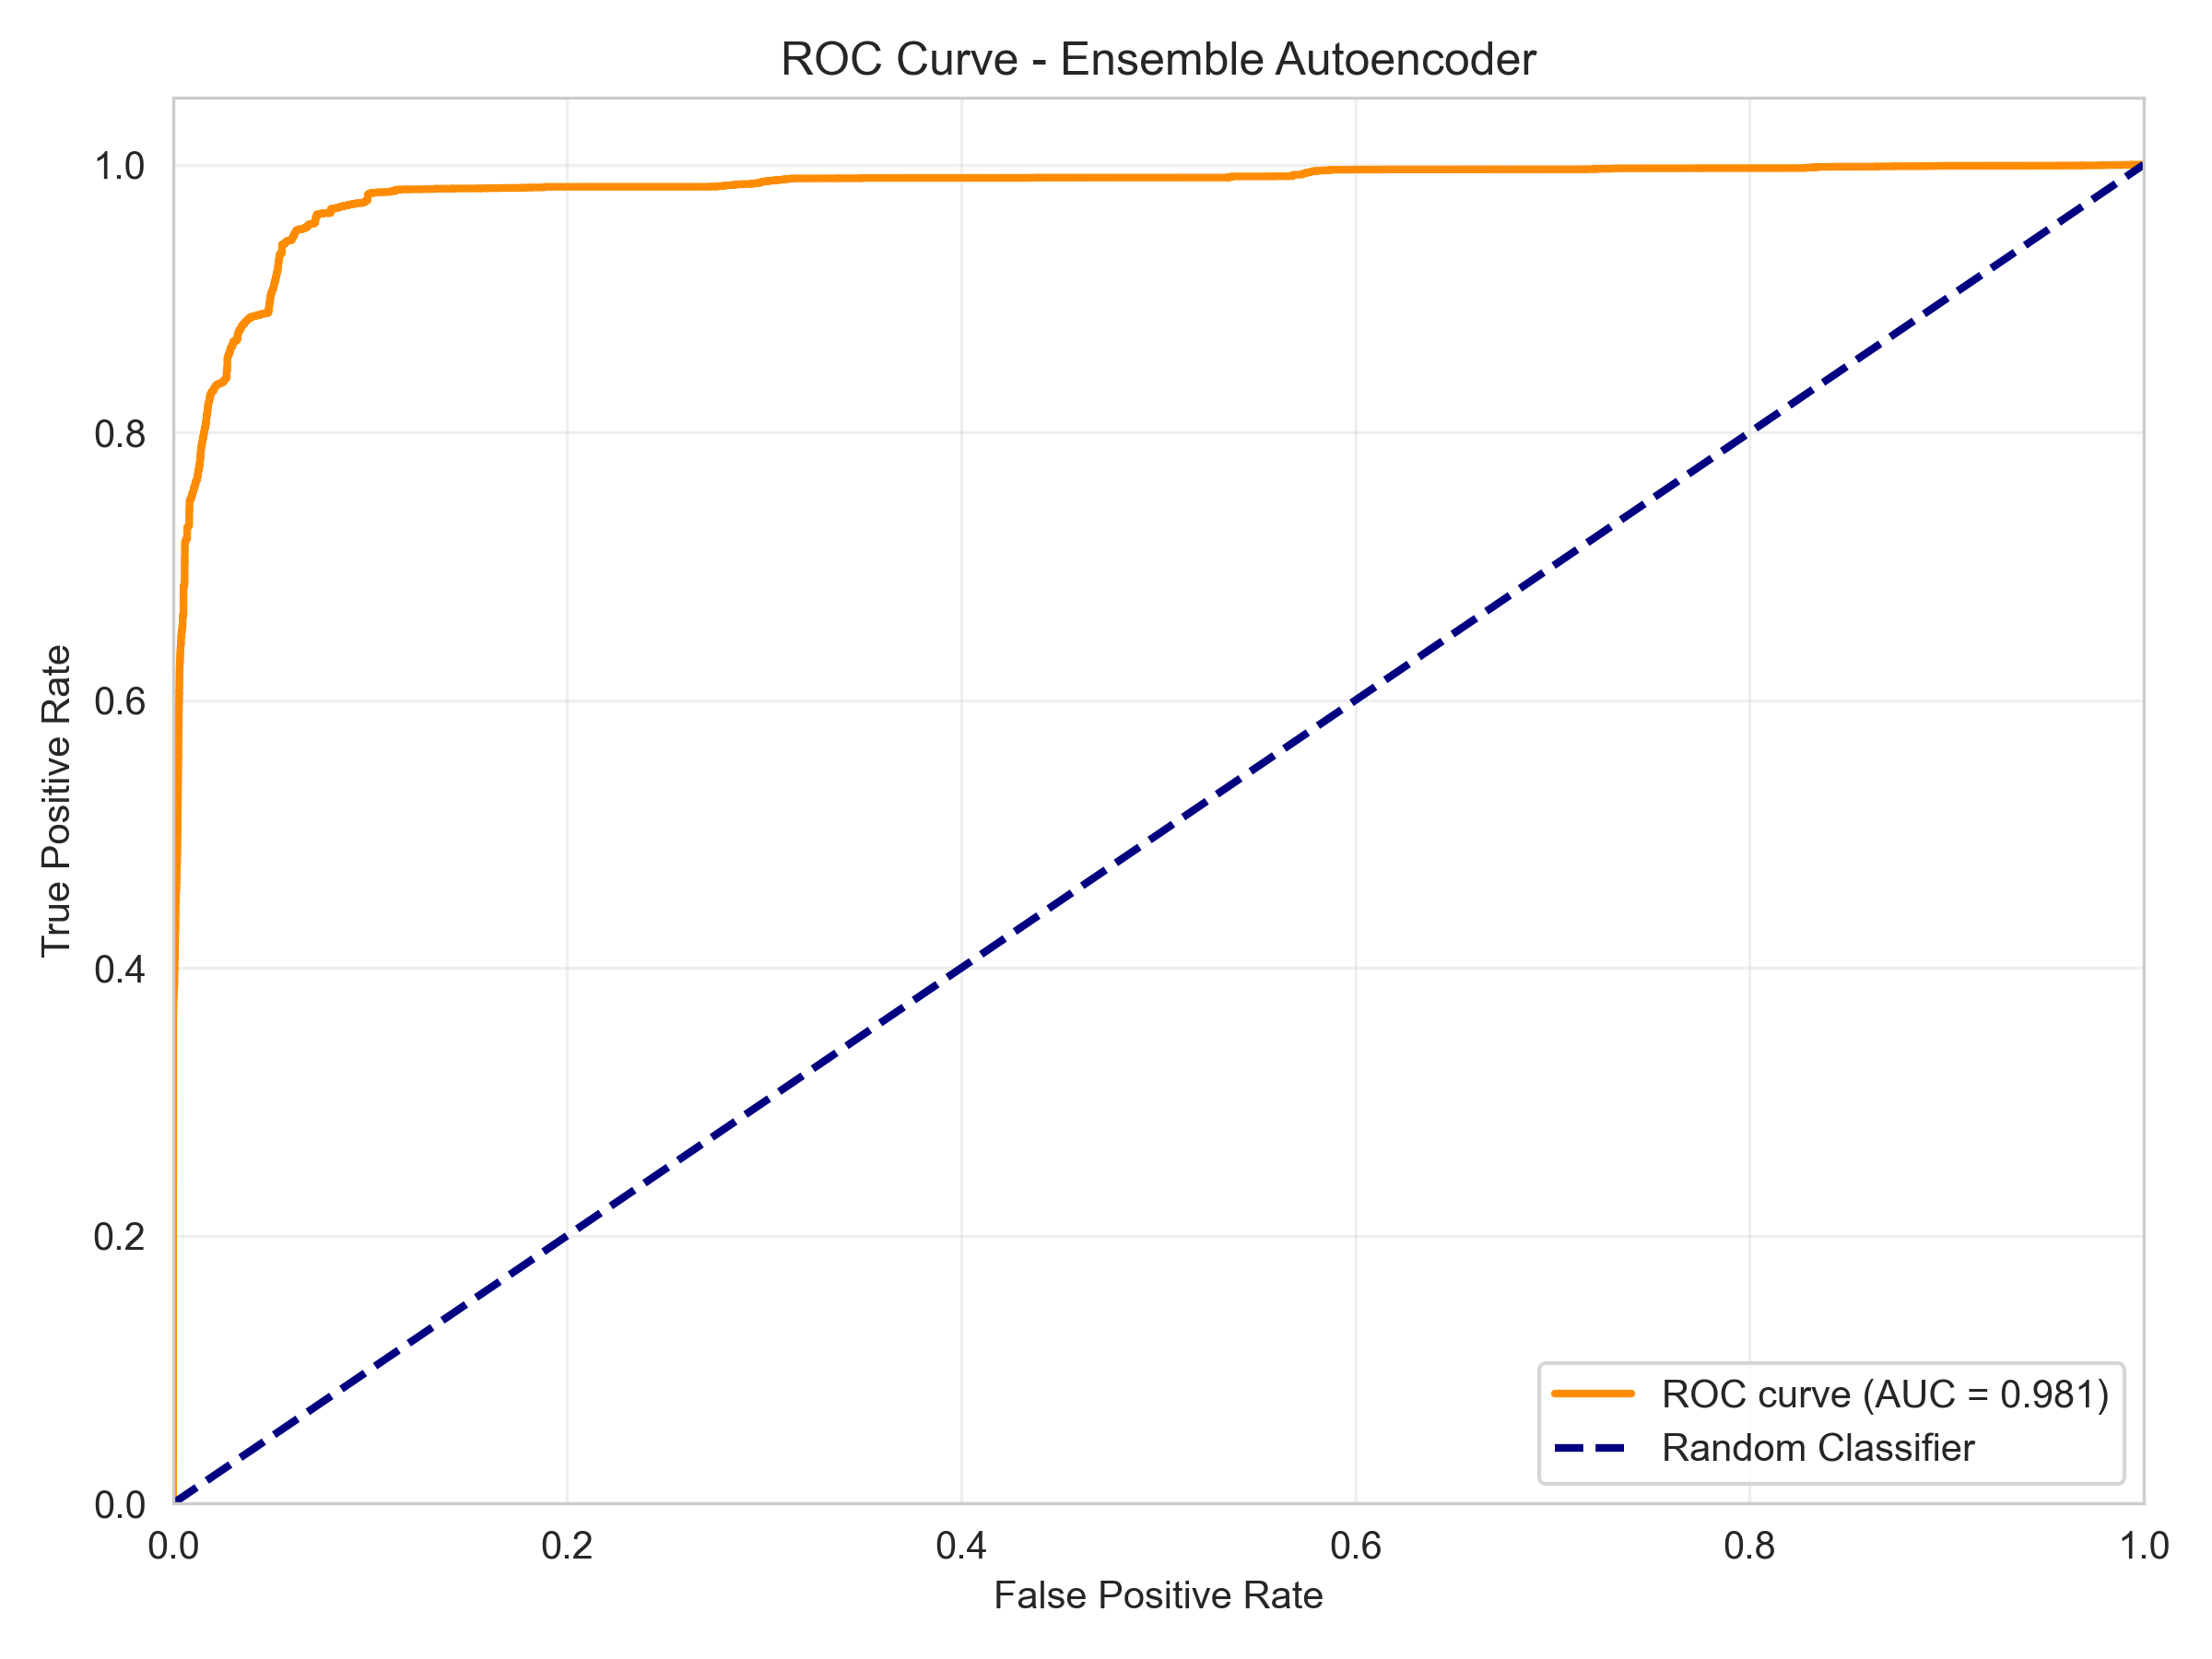
\includegraphics[width=0.85\textwidth]{images/ensemble_autoencoder_roc.png}\\
      \scriptsize{ROC Curve (AUC = 0.981)}
    \end{column}
  \end{columns}
  \vfill
  \begin{itemize}
    \item Out of 16,697 actual anomalies in the test set, only 785 are missed.
    \item The 58.55\% precision is due to the logical OR aggregating false positives, which is an acceptable compromise for security operations.
  \end{itemize}
\end{frame}

\begin{frame}{Overfitting and Underfitting Analysis}
  \begin{itemize}
    \item \textbf{Underfitting}:
    \begin{itemize}
      \item \textit{Local Outlier Factor (LOF):} Underfits severely in 70D because distance concentration hides outlier patterns.
      \item \textit{Baselines:} Isolation Forest and OC-SVM default parameters fail to capture multi-vector attack profiles.
    \end{itemize}
    \item \textbf{Overfitting}:
    \begin{itemize}
      \item \textit{One-Class SVM:} Highly prone to overfitting if $\gamma$ is too high, leading to a tight envelope and massive false alarms.
      \item \textit{Autoencoders:} Prevented from overfitting (identity mapping) by a compact bottleneck architecture ($70 \to 8$).
    \end{itemize}
    \item \textbf{Regularization:} Managed by monitoring train/val loss curves.
  \end{itemize}
\end{frame}

\begin{frame}{Critical Reflection and Responsible AI}
  \begin{itemize}
    \item \textbf{Theory vs. Practice:} In high dimensions, density concepts (like LOF) degrade. Modeling must align with data geometry.
    \item \textbf{Ethical Dimensions:}
    \begin{itemize}
      \item False positives can block legitimate users, impacting business.
      \item Models are trained on university network traffic from 2017; generalizability to modern, zero-day corporate networks requires validation.
    \end{itemize}
    \item \textbf{AI Tools Disclosure:} Used Gemini Pro for debugging PyTorch tensors and Scite.ai/Elicit.com for literature reference verification.
  \end{itemize}
\end{frame}

\begin{frame}{Conclusions and Future Work}
  \begin{itemize}
    \item \textbf{Key Takeaways:}
    \begin{enumerate}
      \item Unsupervised Deep Learning is highly successful for anomaly-based IDS.
      \item Ensemble AE provides maximal security monitoring (95.3\% recall).
      \item Secondary AE minimizes false alarms, suitable for automated mitigation.
    \end{enumerate}
    \item \textbf{Future Work:}
    \begin{itemize}
      \item Integrating Deep Autoencoding Gaussian Mixture Models (DAGMM).
      \item Adding Attention layers inside the encoder/decoder stacks.
      \item Implementing weighted scoring logic instead of strict binary OR.
    \end{itemize}
  \end{itemize}
  \vfill
  \centering \textbf{Thank you. Questions?}
\end{frame}

\end{document}
